
\chapter{Pariticle-In-Cell}
\label{chap:pic}

\section{等离子体数值模拟}
\begin{figure}[!htbp]
  \centering
  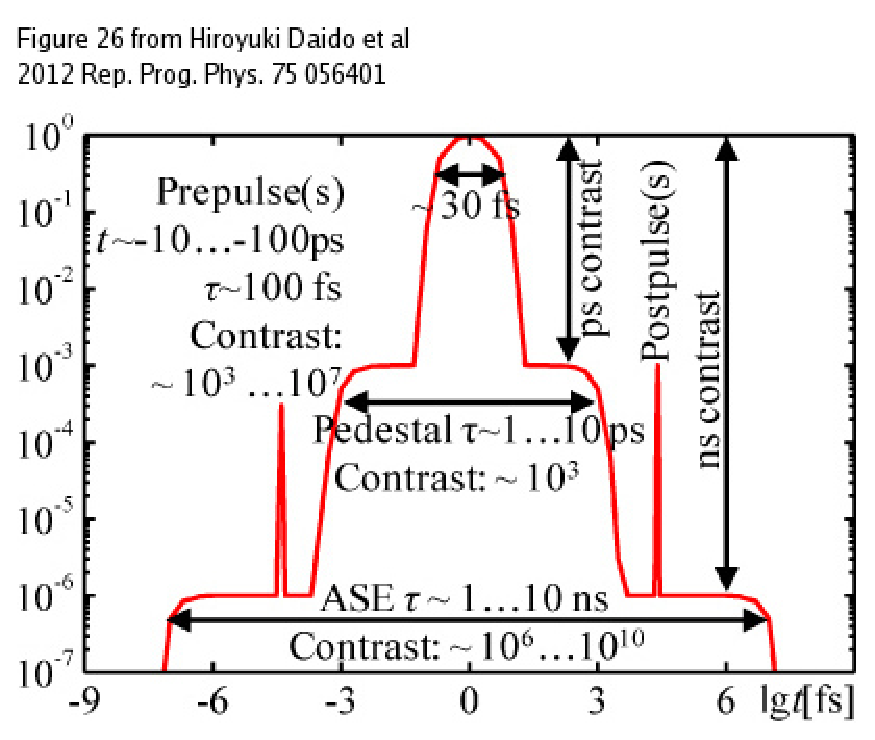
\includegraphics[width=\MyFactor\textwidth]{Img/prepulse2012.eps}
  \caption{激光脉冲示意图}
  \label{fig:prepulse2012}
\end{figure}

激光的相互过程中,设计到波-波、波-粒子、粒子-粒子的相互作
用,是一个多模、多粒子系统的强非线性相互作用过程。解析方法很难全面地进行研究,数值计算就是必然的选择。
数值模拟的方法在激光等离子体相互作用的领域中有重要的意义。首先,模拟工作往往具有前瞻性,许多重要的发现是建立在模拟工作的基础上,对实验提出要求与指导。由于数值模拟的灵活性,实验中难以达到的条件,可以在数值计算中进行模拟,寻找最优解决方法。同时,模拟工作可以解释实验中的新发现,全方位地对于物理过程进行剖析,有助于更好地理解实验现象。实验和模拟之间,互为依靠,相辅相承。现代数值模拟,借助与CPU以及GPU等高速计算工具,以及MPI和CUDA等优秀的计算平台,其计算功能已经相对成熟。
从模拟的算法角度,对于不同对象,模拟中采用不同的数值方法。对等离子体这种呈现集体运动特性的带电粒子的复杂系统(等离子体)的数值模拟研究,一般用流体力学模拟或动理学模拟方法


\subsection{流体力学模拟}


流体力学模拟方法从宏观统计角度研究等离子体特性,例如:温度、密度、压强等,其精度在空间上百微米量级,时间上纳秒量级。其方法,是将微观得到的吸收系数或输运系数的作为已知条件,求解磁流体力学(MHD)方程,得到粒子的分布信息。通过粒子分布函数对参量进行积分,得到统计意义上的结果。
完整的流体力学方程组,可以通过取 Vlasov 方程的不同的速度矩得到:

连续性方程:$\partial{n_j}/\partial{t}+\partial{n_j \bar{\vec{u_j}}}/\partial{t} =0$
运动方程:$n_j \partial {\vec{u_j}}/\partial{t}+n \vec{u_j} \partial{\vec{u_j}}/\partial{\vec{x}} = \frac{n_j q_j}{m_j} ( \vec{E}+\frac{\vec{u_j} \times \vec{B}}{c}) - \frac{1}{m_j} \frac{\partial{\vec{p_j}}}{\vec{x}}$

状态方程:
\begin{equation}
\[ \left\{
  \begin{array}{lr}
    p_j=n_j T_j & : \omega / k ll v_j\\
    \frac{p_j}{{n_j}^{\gamma}}=const & : \omega / k gg v_j
  \end{array}
\right.
\]
\end{equation}



其中,j代表粒子种类,温度$T_j$,热速度 $v_j=(T_j/m_j)^{1/2}$,热压 $P_j$。
$\gamma=(2+N)/N$,N是自由度。加上maxwell方程,以上构成流体力学的完备描述。当 $\omega / k ll v_j$时,服从等温分布,当 $\omega / k gg v_j$时,服从绝热分布。当 $\omega / k = v_j$时,流体方法无法描述热传递过程,需要使用Vlasov方程。因此流体力学的描述方法,适用于热传输速度远大于或者小于系统的变化速率,对于二者相当的情况,其状态方程无法用绝热或者热平衡来近似,因此流体力学方法失效。

\subsection{动力学模拟}


动力学模拟在微观上研究等离子体中的物理过程,考虑粒子在电磁场作用下运动。由于微观系统较大的复杂度,其研究等离子体的空间范围和时间尺度都有限,多用于微型空间中的快速过程。主要
包括两种方法:
(1) 求解动力学方程:
Vlasov 方程:

j类粒子在相空间随时间的分布函数 $f_j(\vec{x},\vec{v},t)$满足:
\begin{equation}
\frac{\partial{f_i}}{\partial{t}} + \vec{v} \cdot \frac{\partial{f_i}}{\partial{\vec{x}}} + \frac{1_j}{m_j}(\vec{E}+\frac{1}{c} \vec{v} \times \vec{B}) \cdot \frac{f_i}{\vec{v}}=0
\end{equation}
它描述高温无碰撞等离子体,如受控热核反应和激光等离子体相互作用。




Fokker-Plank 方程:
描述驰予扩散等非平衡状态的等离子体,在 Vlasov 方程中,加了碰撞项
$\frac{\partial{f_i}}{\partial{t}} + \vec{v} \cdot \frac{\partial{f_i}}{\partial{\vec{x}}} + \frac{1_j}{m_j}(\vec{E}+\frac{1}{c} \vec{v} \times \vec{B}) \cdot \frac{f_i}{\vec{v}}=(\partial{f}/\partial{t})_{collision}$

begin{equation}
\label{eqn:energyCon}
\rho D_t e = -P \nabla \cdot \bf{v} - \nabla \cdot \bf{q} -Q +S
\end{equation} 

利用流体力学方程或动力学方程求解问题时,由于存在一个多维相空间的分
布函数,数值求解时要进行离散化处理,容易产生非物理的多束流失真。因此无
论是流体力学方程还是动力学方程,都需要对作为统计系统的等离子体做了光滑
化的近似,抹去了他们固有的统计起伏,然而这些起伏效应在一定条件下可以发
展成象湍流这样的重要物理现象。



\section{粒子模拟}



等离子体的粒子模拟方法(PIC)起源于上世纪60年代,经过几十年的发展,其功能不断地完善,成为等离子体作用研究中的一种成熟的数值模拟方法。其原理是跟踪计算大量的粒子在自洽场以及外加磁场中的运动,运用统计平均的方法得到电流,密度等宏观量的以及等离子体中的集体效应。有关粒子模拟方法的书籍文献[1-15]。首先介绍PIC中的量纲,计算机模拟过程中,有些物理量非常小,如电子质量、电量、波长等,而有
些量却很大,如光速等,用计算机直接进行这些量之间的加减乘除等计算,非常
不方便,而且很有可能在计算中因变量太大而导致数值溢出或变量太小而导致有
效数字的损失。处于计算方便的考虑,物理量都做了归一化,所以在数值计算中各物理量均采用无量纲量形式:


  $t=t_{real}/{{\omega}_{pe}}^{-1}$,
  
  $x=x_{real}/ {\lambda}_{D}$
  
  $m=m_{phy}/m_e$, $m_e$

  $q=q_{phy}/e$, e

  $n=n_{phy}/n_pe$

  $v=v_{real}/{v_{th}}$
  
  $P=\gamma mv =P_{phy}/{m_e v_{th}}$
  
  $E=E_{phy}/(m_e v_{th} \omega_{pe} /e )$
  
  $B=B_{phy}/(m_e v_{th} \omega_{pe} /e )$
  
  $J=J_{real}/(ev_{th}n_c)$,
  

  
其中, $\omega_{pe}$是初始等离子体频率, $v_{th}=(k_B T_e / m_e)^{1/2}$ 是电子初始热速度, $\lambda_D=v_{th}/ {omega}_p$是等离子体初始德拜长度,$m_e$是电子质量,e是电子电荷量,$\gamma$是相对论因子, $n_c$是等离子体临界密度。
  


 \subsection{麦克斯韦方程求解} 
麦克斯韦方程的求解算法的有限时域差分法(FDTD),

无量纲化的微观麦克斯韦方程组(安培方程及法拉第方程)可以写为:  
\begin{equation}
\label{eqn:maxwell}
\begin{dcases*}
\vec{\nabla} \cdot \vec{E}= 2 \pi \rho
\vec{\nabla} \cdot \vec{B}= 0

\frac{\partial{\vec{E}}}{\partial{t}} = \vec{\nabla} \times \vec{B} - 2 \pi \vec{J}
\frac{\partial{\vec{B}}}{\partial{t}} = -\vec{\nabla} \times \vec{E}
\end{dcases*}
\end{equation}  
对安培方程求梯度,得到:  
${\nabla} \cdot {\partial}_t \vec{E} = c {\nabla} \cdot ({\nabla} \times \vec{B})-{\nabla} \cdot \vec{J}={\nabla} \cdot \vec{J} $, 在电荷守恒${\partial}_t  \rho + {\nabla} \cdot \vec{J} =0 $的条件下, 因此有高斯方程${\nabla} \cdot \vec{E}=\rho $恒成立。同时,如果初始条件有$\vec{\nabla} \cdot \vec{B}_{t=0}=0$, 那么由$\nabla \cdot {\partial}_t \vec{B} = -\vec{\nabla} \cdot \vec{\nabla} \times \vec{E} =0$,得到$\vec{\nabla} \cdot \vec{B}=0$恒成立。

将方程组\ref{eqn:maxwell}的矢量参数转化成标量参数,可得:
\begin{equation}
\label{eqn:maxwell_scale}
\begin{dcases*}

\partial_t {E_x}=(\partial_y {B_z} - \partial_z {B_y}) - 2 \pi J_x
\partial_t {E_y}=(\partial_z {B_x} - \partial_x {B_z}) - 2 \pi J_y
\partial_t {E_z}=(\partial_x {B_y} - \partial_y {B_z}) - 2 \pi J_z
\partial_t {B_x}=(\partial_y {E_z} - \partial_z {E_y})
\partial_t {B_y}=(\partial_z {E_x} - \partial_x {E_z})
\partial_t {B_z}=(\partial_x {E_y} - \partial_y {E_x})

\end{dcases*}
\end{equation} 
  


%%% we need to get the graphic for the yee grid
FDTD算法常采用YEE氏晶格\cite{yee1966numerical}分配电场和磁场在网格上的位置,如图
\ref{fig:yee}所示。方程\ref{eqn:YEE}为基于YEE 氏晶格将微分方程组\ref{eqn:maxwell_scale}的第一个方程转换成
差分方程的形式,其他微分方程方程也可很容易地类似写成相应的差分形式。
基于YEE氏晶格法的FDTD算法在时间和空间上都是中心差分,二阶精度。
\begin{figure}[!htbp]
  \centering
  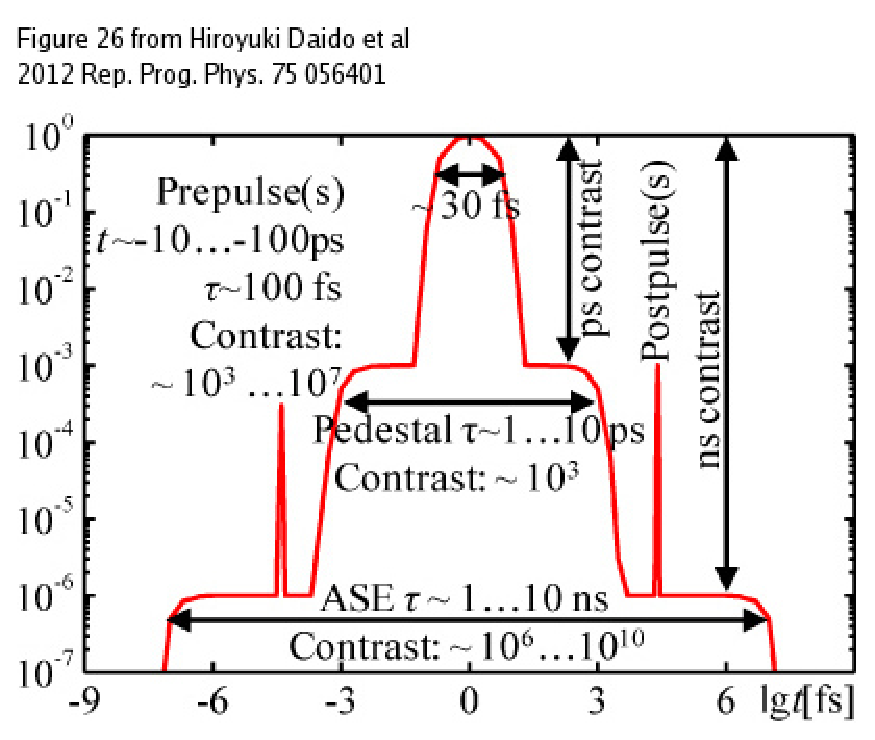
\includegraphics[width=\MyFactor\textwidth]{Img/prepulse2012.eps}
  \caption{YEE氏晶格}
  \label{fig:yee}
\end{figure}

\begin{equation}
\label{eqn:YEE}
\begin{dcases*}

\frac{{E_x}^{n}(i+\frac{1}{2},j,k)-{E_x}^{n-1}(i+\frac{1}{2},j,k) }{\delta t}=  \frac{{B_z}^{n-\frac{1}{2}}(i+\frac{1}{2},j+\frac{1}{2},k)-{B_z}^{n-\frac{1}{2}}(i+\frac{1}{2},j-\frac{1}{2},k) }{\delta y} -  \frac{{B_y}^{n-\frac{1}{2}}(i+\frac{1}{2},j,k+\frac{1}{2})-{B_y}^{n-\frac{1}{2}}(i+\frac{1}{2},j,k-\frac{1}{2}) }{\delta z}- 2 \pi {J_x}^{n-1/2}(i+\frac{1}{2},j,k)

\end{dcases*}
\end{equation} 




实际处理中,综合考虑计算精度计算量等,可以进行一定的简化处理。从研究等离子体问题的性
质上可以分为:
1.静电模:要研究的等离子体的运动主要由于电荷分离产生静电场
引起。如,Langmuir 波,离子声波,双流不稳定性。只求解波松方程
($\vec{\nabla} \cdot \vec{E} = 4 \pi \rho $
)。其特征时间为${\omega_{pe}}^{-1}$,${\omega_{pe}$是静电振荡频率。
2.静磁模:研究磁约束、磁流体(MHD)、阿尔芬波等。求解Maxwell
方程,但略去了位移电流。其特征时间为静电振荡${\omega_{pe}}^{-1}$或电子回旋时间
${\omega_{ce}}^{-1}$。
3.电磁模:求解完整的Maxwell 方程组。其特征时间为$\lambda_D/c$。


同时还可以根据具体问题,将三维程序简化为一维 、二维、
三维,还有1D2V(一个空间分量,两个速度分量)、1D3V(一个空间分量,三个
速度分量)和2D3V(两个空间分量,三个速度分量),从而在保证研究问题的需求精度的基础上大幅度地简化计算的规模。由于本论文的工作大多基于2D3V,因此对于麦克斯韦方程的二维差分形式做以介绍:


对于TM模,Maxwell方程组的二维中心差分形式

\begin{equation}
\label{eqn:maxwell_TM}
\begin{dcases*}

\frac{ {E_x}^{n+1}(i,j+1/2)-{E_x}^{n}(i,j+1/2)}{\delta t} = \frac{ {B_z}^{n+1/2}(i,j+1)-{B_z}^{n+1/2}(i,j)}{\delta y}-2 \pi {J_x}^{n+1/2}(i,j+1/2)
\frac{ {E_y}^{n+1}(i,j+1/2)-{E_y}^{n}(i,j+1/2)}{\delta t} = \frac{ {B_z}^{n+1/2}(i,j+1)-{B_z}^{n+1/2}(i,j)}{\delta x}-2 \pi {J_y}^{n+1/2}(i+1/2,j)

\frac{ {B_z}^{n+1/2}(i,j)-{B_z}^{n-1/2}(i,j)}{\delta t} = \frac{ {E_y}^{n}(i+1/2,j)-{E_y}^{n}(i-1/2,j)}{\delta x}- \frac{ {E_x}^{n}(i,j+1/2)-{E_x}^{n}(i,j-1/2)}{\delta y}

\end{dcases*}
\end{equation} 


对于TE模,Maxwell方程组的二维中心差分形式是:

\begin{equation}
\label{eqn:maxwell_TE}
\begin{dcases*}

\frac{ {E_z}^{n+1}(i+1/2,j+1/2)-{E_z}^{n}(i+1/2,j+1/2)}{\delta t} = \frac{ {B_y}^{n+1/2}(i+1,j+1/2)-{B_y}^{n+1/2}(i,j+1/2)}{\delta x}-\frac{ {B_x}^{n+1/2}(i+1/2,j+1)-{B_x}^{n+1/2}(i+1/2,j)}{\delta x}- 2 \pi {J_z}^{n+1/2}(i+1/2,j+1/2)

\frac{ {B_x}^{n+1/2}(i+1/2,j)-{B_x}^{n-1/2}(i+1/2,j)}{\delta t} = \frac{ {E_z}^{n}(i+1/2,j+1/2)-{E_z}^{n}(i+1/2,j-1/2)}{\delta y}

\frac{ {B_y}^{n+1/2}(i,j+1/2)-{B_y}^{n-1/2}(i,j+1/2)}{\delta t} = \frac{ {E_z}^{n}(i+1/2,j+1/2)-{E_z}^{n}(i+1/2,j-1/2)}{\delta x}

\end{dcases*}
\end{equation} 


\begin{figure}[!htbp]
  \centering
  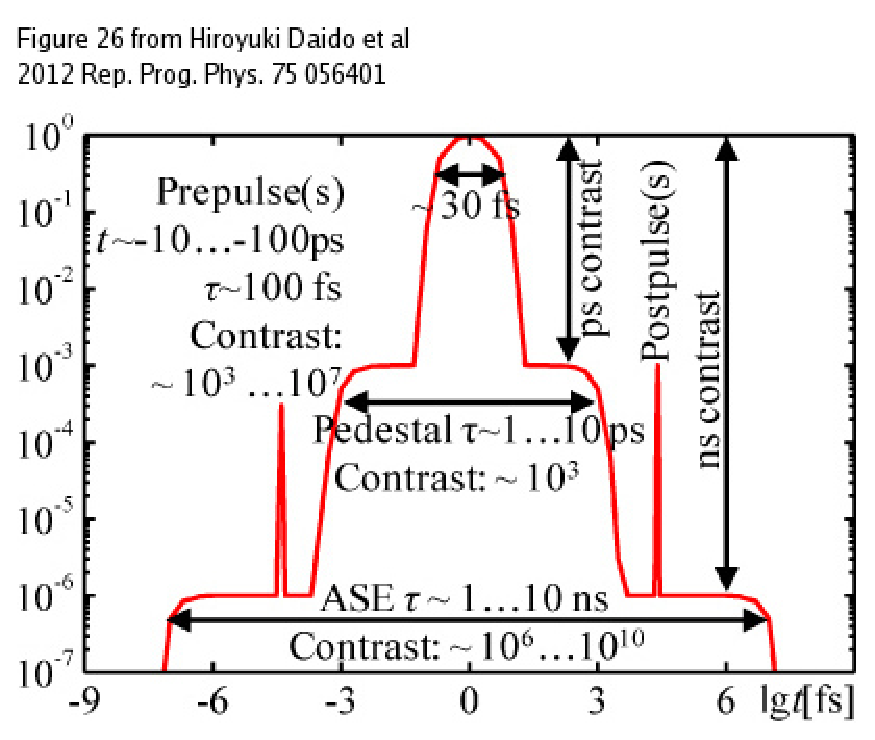
\includegraphics[width=\MyFactor\textwidth]{Img/prepulse2012.eps}
  \caption{YEE氏晶格二维}
  \label{fig:yee2d}
\end{figure}



其中空间步长$\delta x=\delta y=\delta$,时间步长$\delta t= \delta /2$,时间步长和空间步长应满足courant
条件:$(c \delta t)^2 [1/(\delta x)^2 + 1/(\delta x)^2] < 1$。可见,每个电磁分量的值只和它自己上个时刻的值,以及和它最近邻点上的
电磁分量的上半个时刻的值有关系。这有利于实现程序的并行化。


\sbusection{粒子运动的求解}

%%%%%%%%%%%%%%%we need to add the citation to 
%%%%%%%J. P. Boris, in Proceedings of the 4th Conference on Numerical Simulation of Plasma.
Plasmas (Naval Res. Lab, Washington, D.C., 1970),pp. 3.
粒子运动的求解和麦克斯韦场的求解交替进行的。粒子的运动改变场分布,场信息的更新进一步促使粒子运动。PIC中使用半加速-旋转-半加速方法解(无量纲化)相对论粒子运动方程
   
\begin{equation}
\label{eqn:PIC_motion}

m \frac{d \vec{u}}{dt}=2 \pi q (\vec{E} + \frac{\vec{u}}{\gamma} \times \vec{B})
\frac{d \vec{r}}{dt}= \vec{v}

\end{equation} 


其中$\vec{u}=\gamma \vec{v} = \vec{v}/\sqrt{1+ {\vec{v}}^2}$,$\gamma$是粒子的相对论因子。将运动方程化成差分形式


\begin{equation}
\label{eqn:PIC_motion_derivative}
\begin{dcases*}

\frac{\vec{u}^{n+1/2}-\vec{u}^{n-1/2}}{dt}=\frac{2 \pi q }{m} (\vec{E}^n + \frac{\vec{u}^{n+1/2}+\vec{u}^{n-1/2}}{2\gamma} \times \vec{B}^n)
\frac{\vec{r}^{n}-\vec{r}^{n-1}}{dt}= \vec{v}^{n+1/2}

\end{dcases*}
\end{equation} 


做如下替换
\begin{equation}
\label{eqn:PIC_half_acceleration}
\begin{dcases*}

\vec{u}^{n-1/2} = \vec{u}^{-}- \frac{\pi q }{m} \vec{E}^n \delta t
\vec{u}^{n+1/2} = \vec{u}^{+} +\frac{\pi q }{m} \vec{E}^n \delta t

\end{dcases*}
\end{equation} 

,上式转化为
\begin{equation}
\label{eqn:PIC_half_acceleration}
\begin{dcases*}

{\vec{u}^{+}-\vec{u}^{-}}=\frac{2 \pi q }{m} \frac{{\delta} t}{2 {\gamma}^n} {\vec{u}^{+} + \vec{u}^{-}} \times \vec{B}^n)
\end{dcases*}
\end{equation} 


进一步,$\vec{t}= \frac{2 \pi q}{m} \frac{{\delta} t}{2 {\gamma}^n} \vec{B}^n$,$\vec{s}=\frac{2\vec{t}}{1+t^2}$,可得


\begin{equation}
\label{eqn:PIC_half_acceleration1}
\begin{dcases*}

\vec{u}^{'}=\vec{u}^{-} + \vec{u}^{-} \times \vec{t}
\vec{u}^{+}=\vec{u}^{-} + \vec{u}^{'} \times \vec{s}

\end{dcases*}
\end{equation} 




\begin{equation}
\label{eqn:PIC_half_explain}
\[
 \vec{u}^{n-1/2} \xrightharpoondown[在前\delta/2时间内]{\vec{E}^n 作用,加速} \vec{u}^{-} \xrightharpoondown[]{\vec{B}^n 作用,旋转} \vec{u}^{+} \xrightharpoondown[在后{delta t}/2时间内]{\vec{E}^n 作用,加速} I \vec{u}^{n+1/2} 
 
 \]
\end{equation}


\begin{figure}[!htbp]
  \centering
  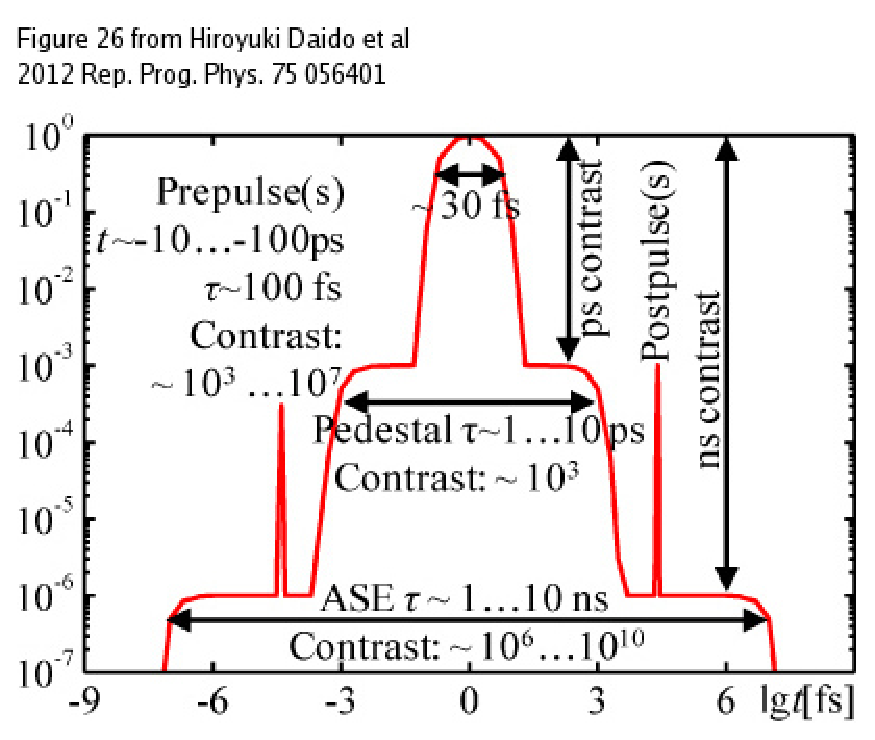
\includegraphics[width=\MyFactor\textwidth]{Img/prepulse2012.eps}
  \caption{Boris半加速半旋转方法}
  \label{fig:}
\end{figure}

   




   
   
   
   
 
   
   
         




粒子模拟方法是从微观角度研究等离子体的某一小区域(例如几百电子
Debye 波长)和较短的时间范围(几百电子等离子体频率)。实际等离子体粒子
数(一个德拜球内的粒子数几千到几万个)虽然比计算机所能模拟的粒子数(一
个德拜球内的粒子数几个到几十个)远大的多,但在等离子体分布函数的相空间
中的一点(x,v)的周围,每个带电粒子对电磁场的贡献和电磁场对粒子的作用
力都基本相同,故周围这些大量带电粒子的运动规律基本相同,因而只用一个粒
子---“超粒子”代表这些粒子的就可以了。这与我们常常只对大于 Debye 长度
的无碰撞等离子体的集体效应感兴趣是一致的,而且我们也并不对所有这些模拟
粒子中的两两相互作用进行计算,而是直接计算空间中的场对模拟粒子的作用。
“超粒子”的引入使得计算机对等离子体做统计计算成为可能。对等离子体做整体量纲分析,可看出,超粒子体系除了 Debye 球内的粒子数目 N d 缩小 N 倍外,所
有基本物理量都不变







\section{粒子受力插值}
要求解粒子运动方程\ref{{eqn:PIC_half_explain},首先得知道作用在粒子位置的电场和磁场大
小,即粒子的受力情形。在PIC 模拟中,场值分布在网格格点上,而粒子可能
分布在模拟空间的任意位置,所以必须将格点上的场值内插到粒子位置,获得
正确的粒子受力,否则在计算中将带来很大的数值噪声和误差。为解决这一问
题,PIC 将计算粒子假设为具有一定形状的分布,而非一个质点。这样,按照
给定的分布函数可以将粒子的宏观属性如电荷,密度,产生的电流等分布在网
格格点上,与场值的位置一样,因此便可更接近得知粒子的受力情形。在PIC
模拟中,因为计算粒子并非一个质点,而是具有一定形状的分布,所以也称之
为虚拟粒子。

\begin{equation}
\label{eqn:current_interpolate}
\begin{dcases*}

q\vec{E}^t=q \sum_p W_p(x){\vec{E}_p}^t
q\vec{B}^t=q \sum_p W_p(x){\vec{B}_p}^t

\end{dcases*}
\end{equation} 



其中$W_p(x)$为处于x位置的粒子在网格点$x_p$的电荷分量,即电荷分布函
数,$W_p(x)$必须满足电荷守恒,匀滑性好等特点。阶数越高,插值力越匀滑,数值噪声越小。接下来给出一个示例如何求解
1D 二阶电荷分布函数(TSC)$W_p(x)$

粒子电荷分布函数$W_p(x)$在其最邻近的三个网格点(−1, 0,1)可以写成二
次方程形式:

\begin{equation}
\label{eqn:charge_distribution}
\begin{dcases*}


W_0(x)=ax^2+b
W_1(x)=W_{-1}(-x)=cx^2+dx=e


\end{dcases*}
\end{equation} 

其中粒子的位置x计算为拉格朗日步长,其定义域为$-1/2<x<1/2$。为计
算方程组\ref{eqn:charge_distribution}的待定系数,考虑粒子处于特殊位置x = 1/ 2,则有:

\begin{equation}
\begin{dcases*}


W_0(1/2)=1/2
W_1(1/2)=1/2
W_(-1)(1/2)=0
\frac{d}{dx} W_{-1}(1/2)=0
\frac{d}{dx} W_{1}(1/2)=-\frac{d}{dx} W_{0}(1/2)

\end{dcases*}
\end{equation} 



\begin{equation}
\begin{dcases*}


a=-1
b=3/4
c=1/2
d=1/2
e=1/8

\end{dcases*}
\end{equation} 

所以粒子电荷分布函数$W_p(x)$可以写成:

\begin{equation}
\begin{dcases*}


W_0(x)=-x^2+3/4
W_1(x)=W_{-1}(-x)=(x+1/2)^2/2


\end{dcases*}
\end{equation}




根据位移不变性原理,$W_p(x)$也可以重写为:

\begin{equation}
\begin{dcases*}


\[
 W(x) =
  \begin{cases}
   \3/4-x^2 & \text{if } (|x| \leq 1/2) \\
   (3/2-|x|)^2/2 & \text{if } (1/2 \geq |x| \leq 3/2) \\
    0 & 其他
  \end{cases}
\]


W_0(x)=3/4-x^2   &&
W_1(x)=W_{-1}(-x)=(x+1/2)^2/2  &&

0 && 其他


\end{dcases*}
\end{equation}


其他任意阶的电荷分布函数$W_p(x)$可以通过同样的方法计算。
将1D 的$W_p(x)$扩展为2D或3D的形式也很简单,只需先分别计算各维度
粒子在其附近网格点的电荷分布情况,然后对各维度的电荷分量对应相乘即得
到最终的电荷分布。以2D TSC 分布函数为例,每个计算粒子的电荷将分布在
其最邻近的$3^2=9$个网格点上,假设$W_i$和$W_j$分别为粒子在x和y方向上最邻近
三个网格点的电荷分布,则2D 电荷分布函数可以写成:
\begin{equation}
W_{ij}=W_{i}W_{j}
\end{equation}
2D TSC 的粒子电荷分布函数及0~4 阶粒子分布所占用网格数可以形象地:




\subsection{电流密度计算}

由连续方程${\partial}_t \rho = - \vec{\nabla} \cdot \vec{J}$可知,带电计算粒子的运动将会产生局部电流,而这局部
电流可以近似为麦克斯韦方程求解的电流项。因为在数值计算粒子运动方程中,所得的粒子速度有一定的误差,所以由
简单的面积平均法求解电流密度分布$\vec{J}=en\vec{v}$并不能严格满足连续方程,
而需求解泊松方程对电场进行修正[55],这需要长程计算,并不易于并行优
化。但若计算该局部电流的过程中满足电荷守恒的条件,则可以避免求解泊松
方程。由连续方程可知,电流密度可由粒子的电荷密度分布变化表征。在
PIC 模拟中,计算粒子并非一个质点,而可以定义为其宏观属性如电荷,密
度,产生的电流等在网格格点上的分布,该分布取决于给定的插值函数和粒子
的位置,而与粒子速度无关。所以局部电流密度的计算将变得非常简单: 只需求
解计算粒子在其附近网格格点上前后时刻的电荷密度分量,再由各格点的电荷
密度变化率即可得该格点的电流密度。假设某粒子$t_0$和$t_1$时刻在其附近网格点
的电荷密度分布分别为矩阵$W_0$和$W_1$,则各网格点的电荷密度变化为:

\begin{equation}
T=W_1-W_0
\end{equation}

则对应产生的电流密度变化$\delta J$为:

\begin{equation}
\delta J =\frac{q}{V} \frac{\delta x}{\delta t} T = \frac{q}{V} \frac{\delta x}{\delta t}(W_1-W_0)
\end{equation}


图  给出了2D TSC 粒子电荷分布函数在单个时间步长内变化产生电流
密度的示意图。值得注意的是,为抑制数值加热,电荷密度分布的变化必须很
匀滑,因此可以采用高阶分布函数。在电荷
守恒的条件下,J. Villasenor 和O. Buneman 给出了基于一阶电荷分布CIC 的电
流密度计算方法[56],但因考虑到各种边界情形,其计算形式非常复杂。而后T.
Z. Esirkepov 给出了任意阶电荷分布函数下电流密度计算的统一形式[57],该形
式可以直接用于PIC 编程中。




\subsection{结论}
